\documentclass[14pt]{article}
\usepackage{graphicx}
\usepackage[left=3cm, right=1.5cm, top=1.5cm, bottom=2cm]{geometry}
\usepackage[russian]{babel}
\usepackage[T2A]{fontenc}
\usepackage[utf8]{inputenc}
\usepackage[unicode]{hyperref}
\usepackage{a4wide}
\usepackage{pdfpages}

\begin{document}

\includepdf[pages=-]{title_Ali.pdf}
\clearpage
\tableofcontents
\clearpage
\section{Команда}
\section{Ресурсы}
	\subsection{Сетевой график}
	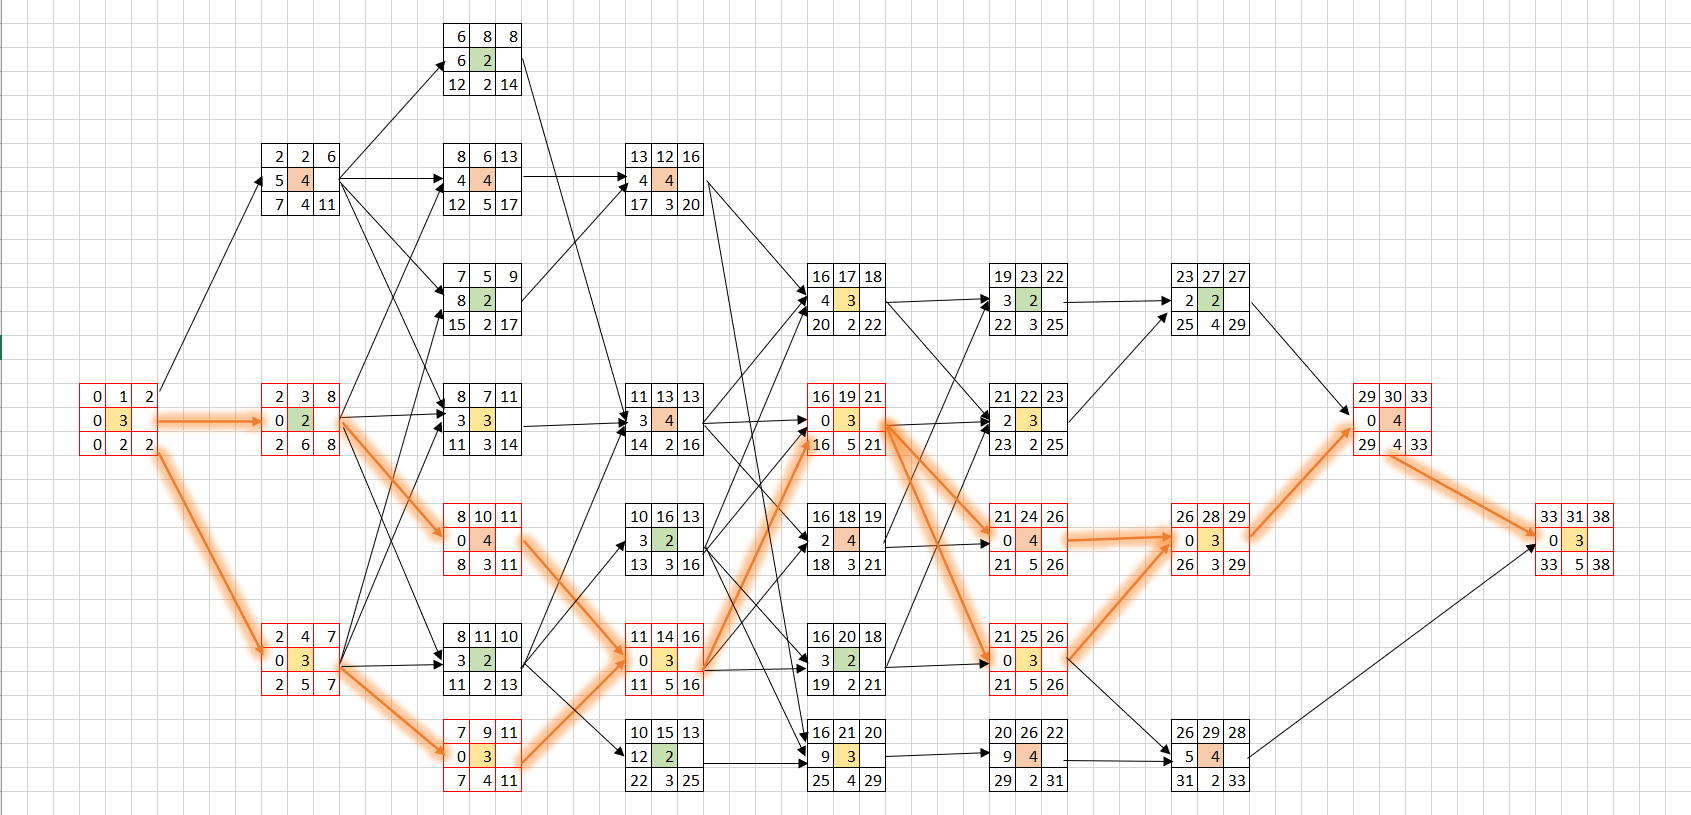
\includegraphics[width=\textwidth]{../img/init_network_graph.png}\\
	В проекте 4 попарно различных кретических пути.
	\subsection{Назначение ресурсов}
	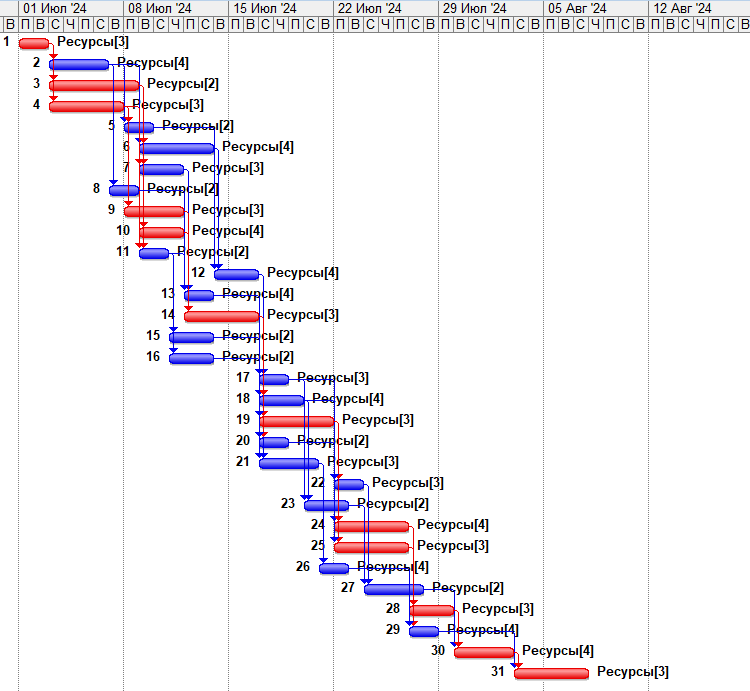
\includegraphics[width=\textwidth]{../img/init_resource_manage.png}
\section{Задача}
	Попробовать уменьшить количество используемых ресурсов до 5 в день, меняя при этом длительность работ не более чем на 2 дня.
	Дату окончания проекта менять нельзя.
\section{Анализ задачи}
	\subsection{Грубый анализ}
		Апроанализируем данные о каждоой задаче.
		
		Вобьём на \texttt{MS Project} данные.
		Уменьшим продолжительность всех задач на 2 дня, где это возможно.
		\texttt{MS Project} за наспочитает дату и время начала и конца каждой задачи.
		Заменим дату конца последней задачи так, чтобы не менять дату окончания проекта.
		Полученные данные скопируем их в \texttt{Excel} и найдём самое раннее начало,
			самый поздний конец и суммарное количество ресурсов.
		Сначала выделит количество дней и резурсов в удобный для чтения формат.
		Далее для каждой задачи посчитаем сколько вообше она потратит ресурсов за период своей обработки.
		Суммируя по всем задачам полученные значения мы получим общее количество ресурсов, необходимых проекту.
		Посчтаем время, которое отведено проекту (в рабочих днях).
		
		Мы можем посчитать средние затраты ресурса на период реализации проекта.
		Так же это значение является ограничением максимального показателя затратов на ресурсы за все дни:
		Если мы всегда тратим меньше ресурсов, чем средние затраты ресурсов, то мы не потратим все ресурсы в указанный период.
		Значит некоторые задачи мы не сделали.\\
		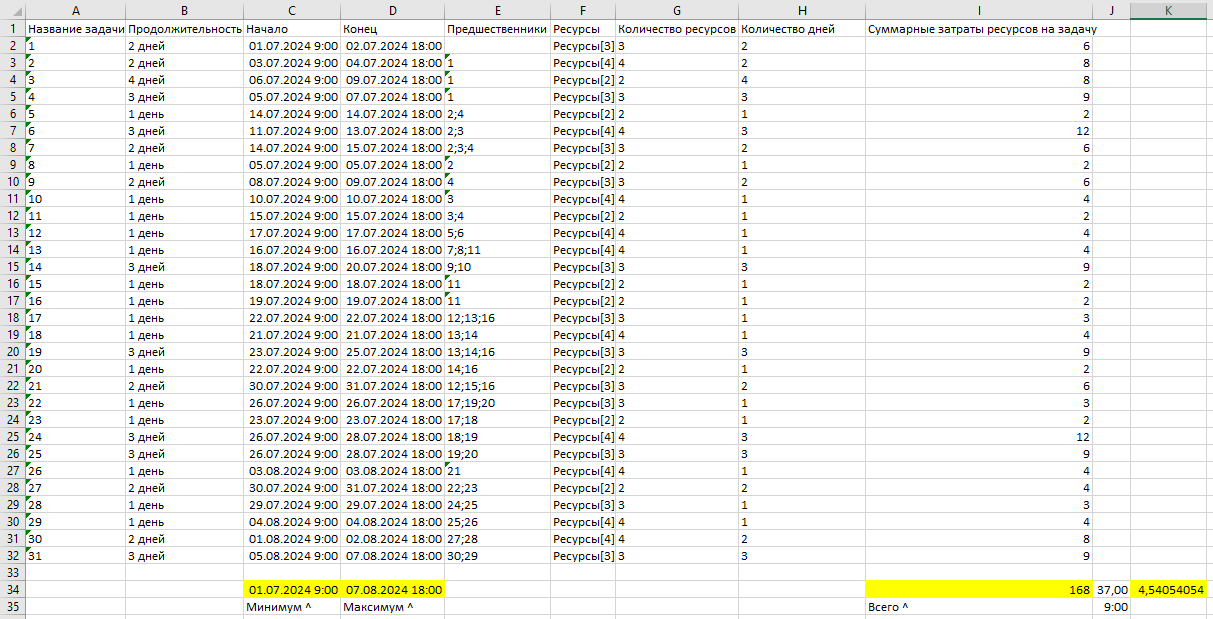
\includegraphics[width=\textwidth]{../img/1a1_time_estimation.png}\\
		Наши рассуждения привели нас к числу $4.5$.
		Это означает, что, ограничиваясь четырьмя ресурсами, мы не сможем реализовать проект.
	\subsection{Анализ, с учётом топологии задач}
		Посмотрим на сетевой график проекта.
		
		По нему видны 2 особые задачи:
		
		Первая -- задача №1 -- задача начала проекта.
		Если она не начнётся, то не может начаться никакая другая задача.
		
		Вторая -- задача №31 -- задача завершения проекта.
		После наступления её даты окончания никакая друга задача не может начаться.
		
		Эти две особые задачи имеют довольно интересное свойство.
		Они не могут выполняться паралельно с любой другой задачей.
		
		Это означает, что мы можем их не учитывать при оценке среднего значения затрат ресурса.
		Вычтим из общих затрат затраты на эти <<особые>> задачи и сузим период.\\
		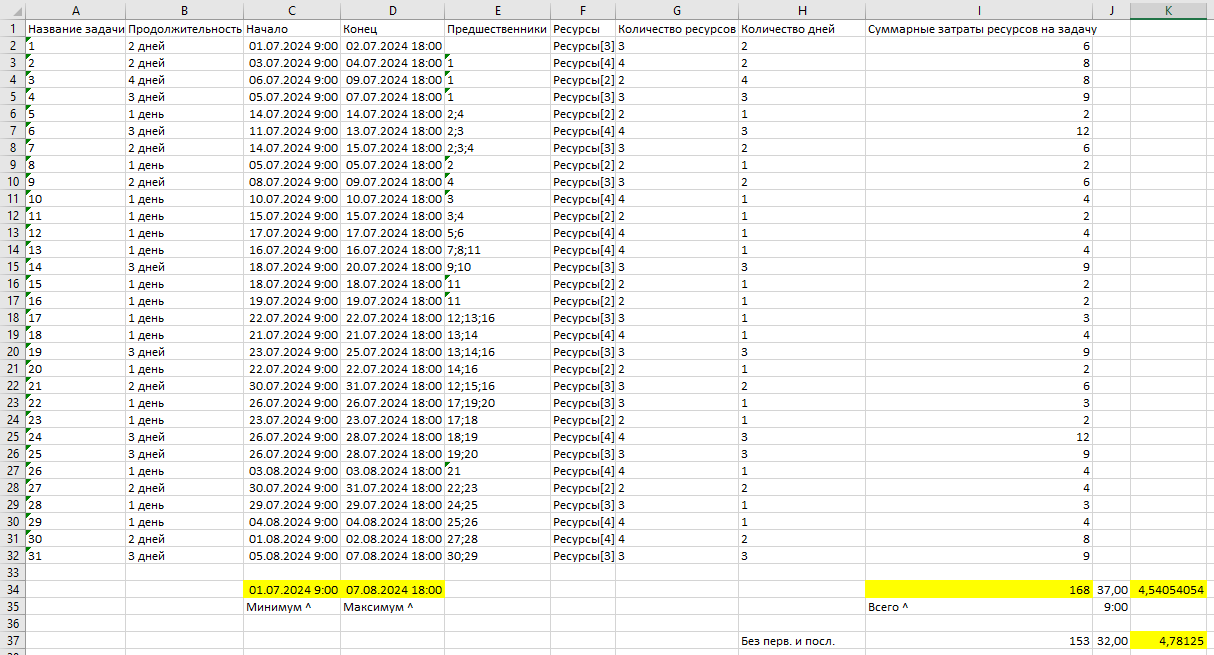
\includegraphics[width=\textwidth]{../img/1a2_time_estimation.png}\\ 
		Опять разделим одно число на другое и получим $4.8$.
		Это ближе к пяти, но пока никаких новых выводов не появилось.
	\subsection{Анализ, с учётом ограничения на ресурсы}
		Известно, что наша цель -- уменьшить затраты ресурсов до величины в 5 ед./день.
		
		Посмотрим внимательно на задачи, чей ресурс равен 4.
		Назовём для краткости такие задачи Четвёрками.
		Раз в списке задач нет такой, чьи затраты небольше единицы, то Четвёрки не могут идти паралельно с какой-нибудь другой задачей.
		Тогда к Четвёркам можно применить те же рассуждения, что и на <<особые>> задачи.
		
		Выделим общие затраты и продолжительность Четвёркок от остальных.\\
		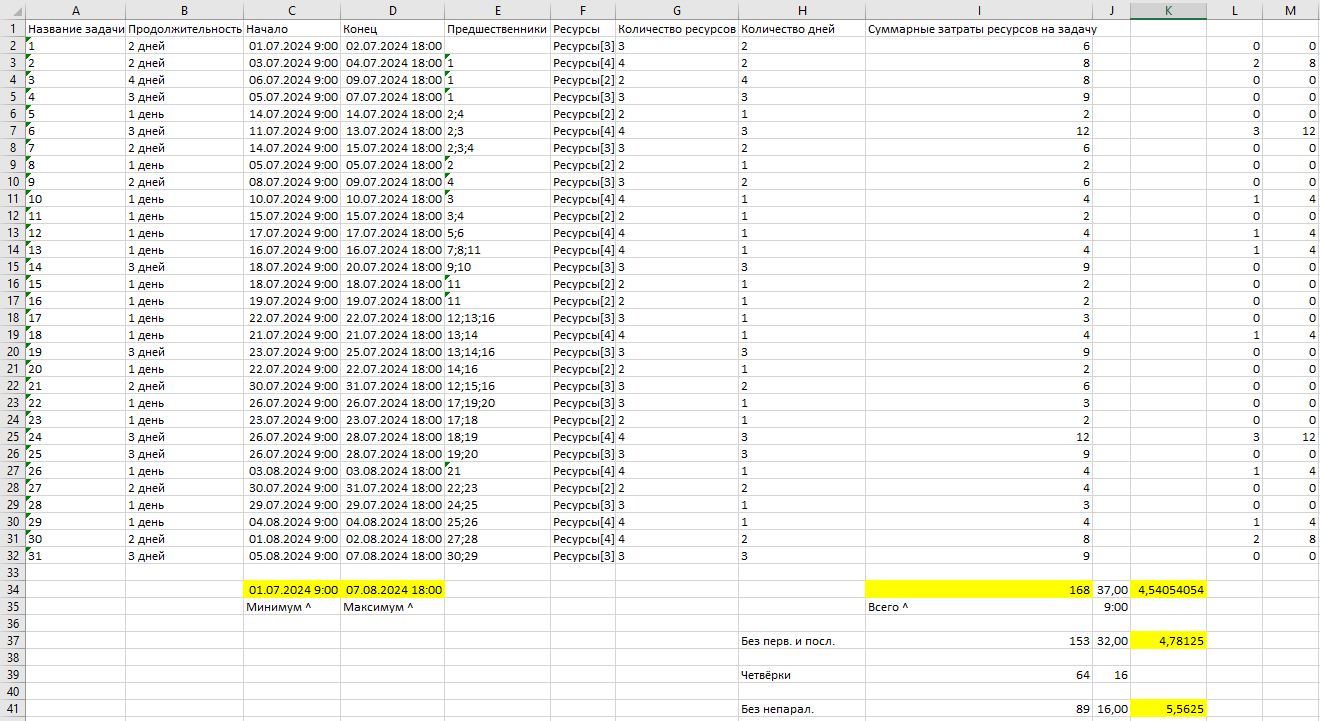
\includegraphics[width=\textwidth]{../img/1a3_time_estimation.png}\\ 
		
		Теперь попробуем посчитать среднее количество затрат для оставшегося промежутка.
		Вычтем из затрат без <<особых>> задач затраты на Четвёрок.
		Также вычтем общего периода существования проекта те участки, которые будут отведены на выполнение задач-Четвёрок.
		Итого, среднее значение получилось $5.6$, что больше пяти.
		Это доказывает, что ограничиваясь пятью ресурсами невозможно реализовать этот проект.
\section{Решение}
	Постараемся найти 3 решения для нашей задачи с учётом проведённого мной анализа.
	\subsection{Первый вариант}
		Первая попытка расставить на места была довольно удачной, хотя пришлось почти все задачи затронуть.\\
		{\LARGE Что поменяли:}\\
		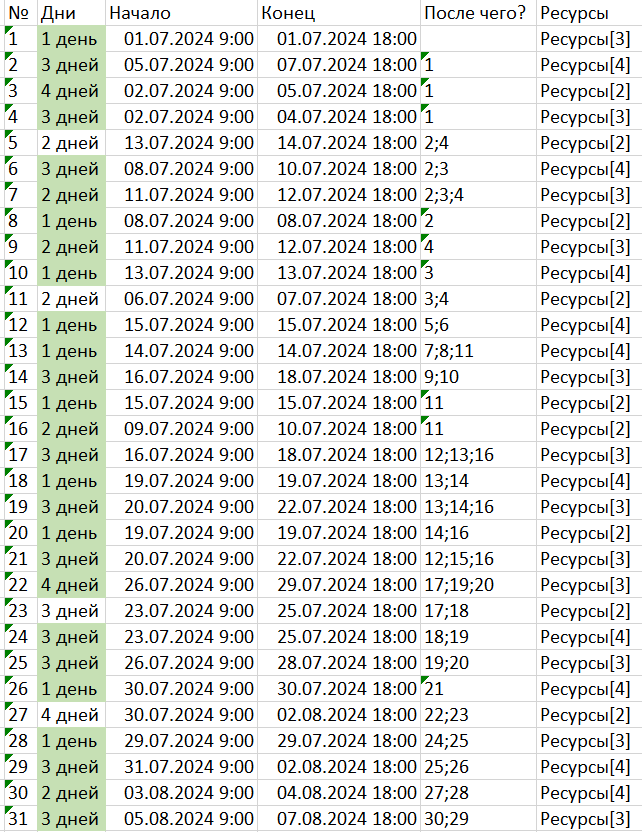
\includegraphics[height=0.6\textheight]{../img/1a1_days_change.png}\\ 
		Внешне диаграмма Ганта стала выглядеть менее структурированной.
		Но это плата грамотному распределению ресурсов.\\
		{\LARGE Как это выглядит:}\\
		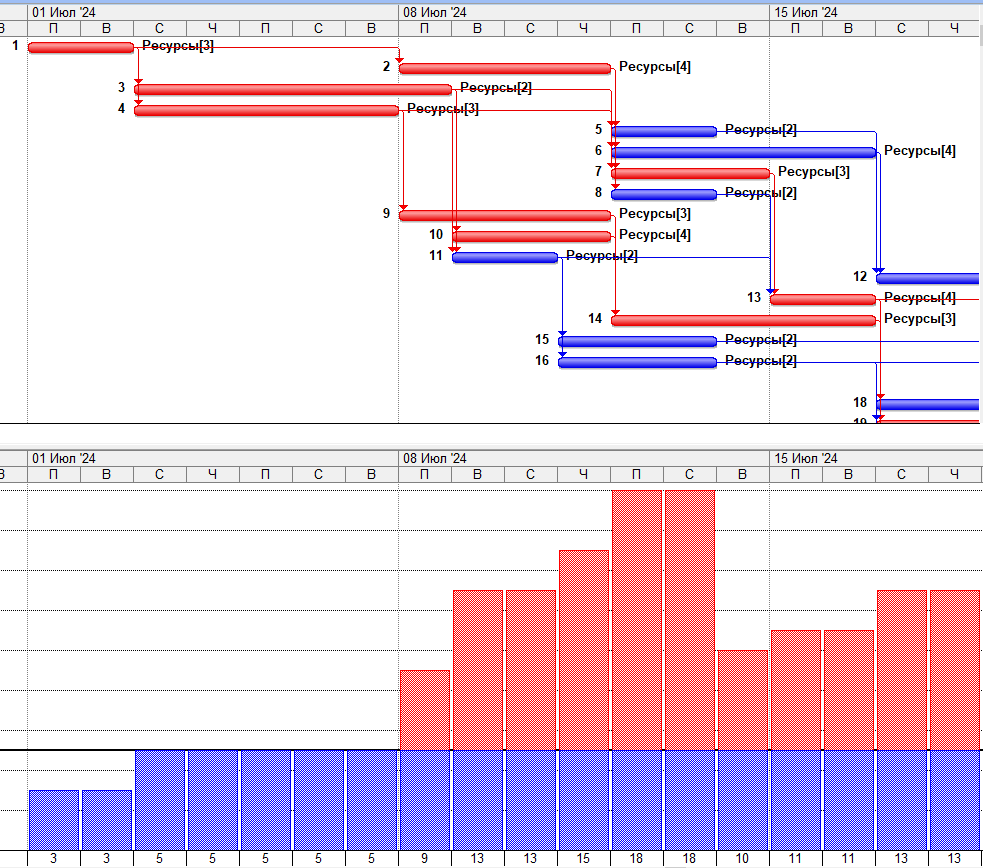
\includegraphics[width=\textwidth]{../img/ot1a1_1.png}\\ 
		С помощью встроеноо функионала напечатаем затраты ресурсов.\\
		{\LARGE Сколько оно тратит:}\\
		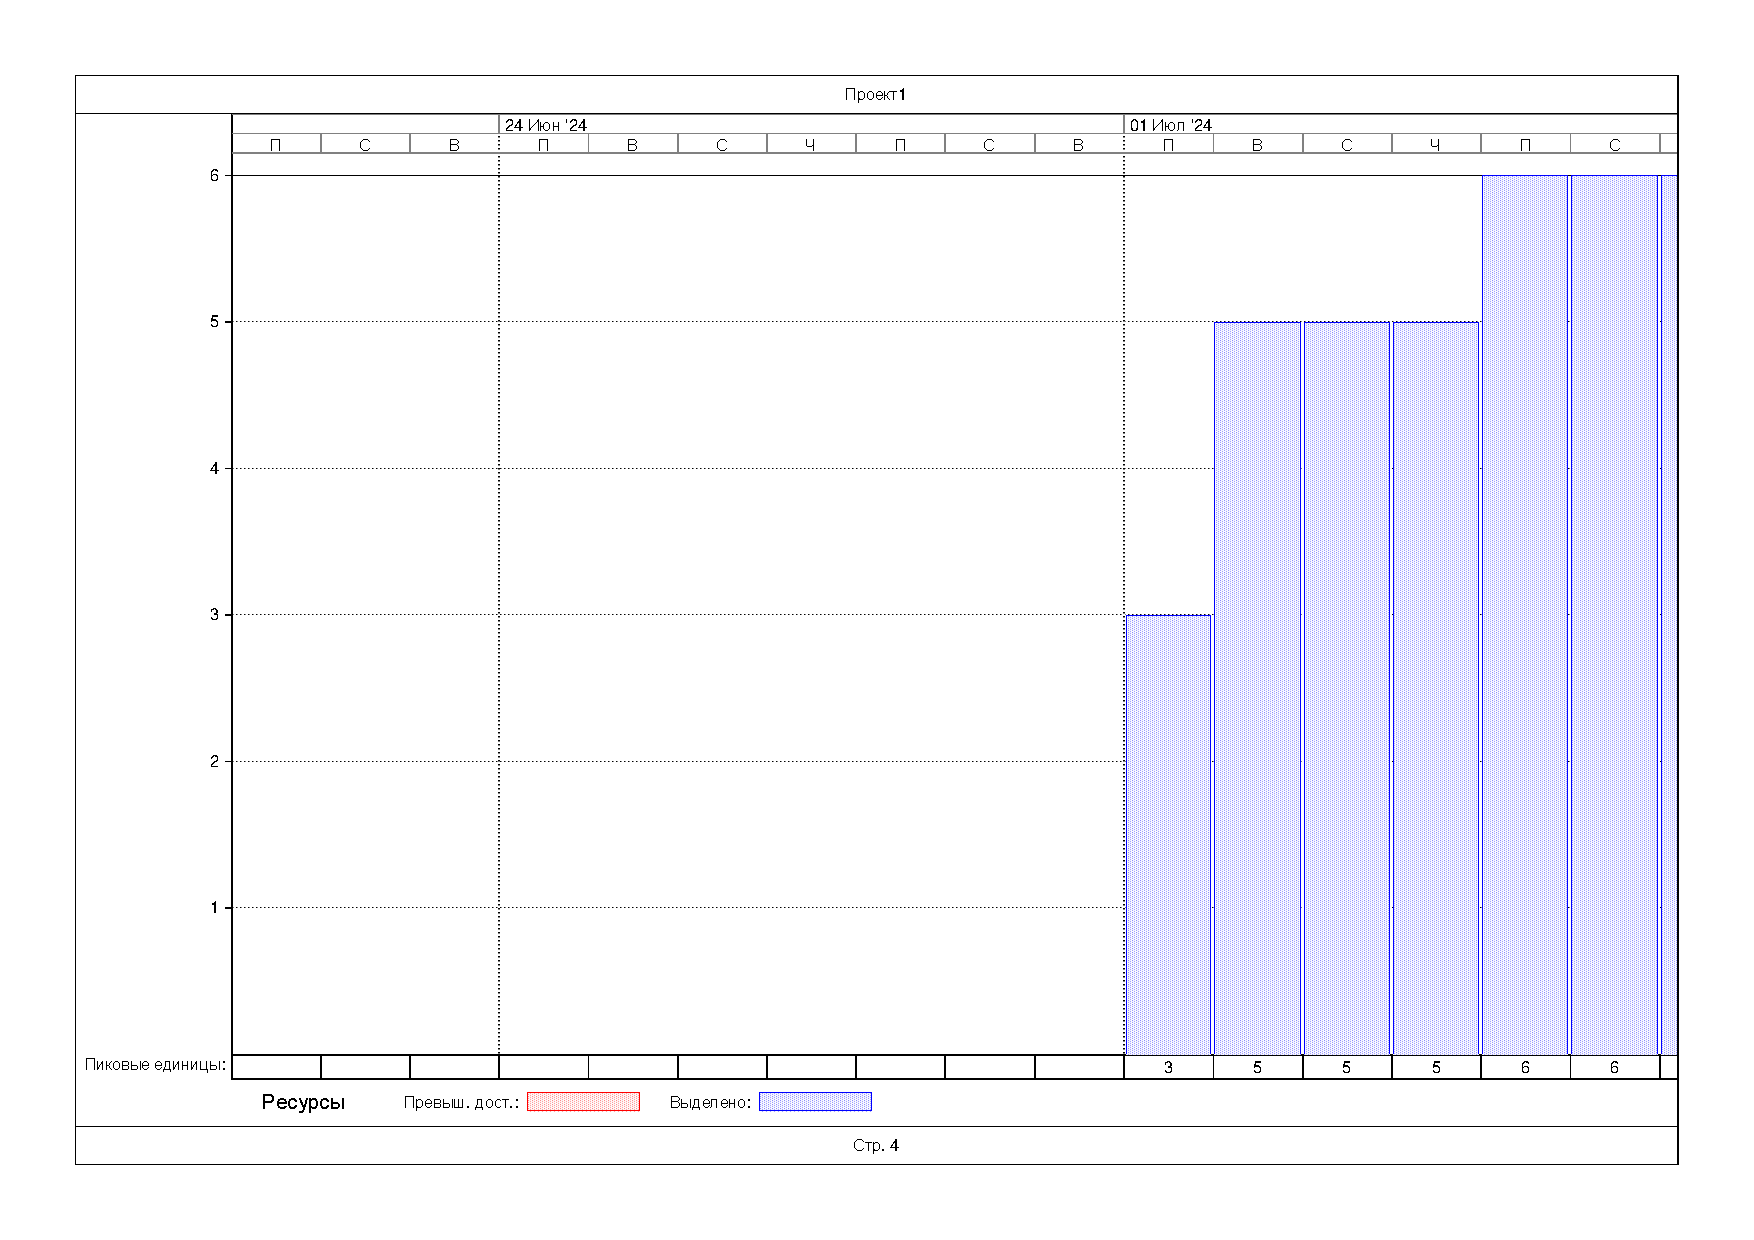
\includepdf[pages=-]{MSOP_Project_ans_1a1.pdf}
	\subsection{Второй вариант}
		Попробуем найти другое решение, чтобы количество изменений было поменьше.
		Конечно, невозможно просто уменьшить число правок.
		Для этого потребуется место, которое можно получить из задач, уменьшенных на 1 день.
		
		Мы сократили количество изменений с 27-ми до 25-ти.
		Дальнейшее улучшение даже если воможно, то крайне затруднительно.\\
		{\LARGE Что поменяли:}\\
		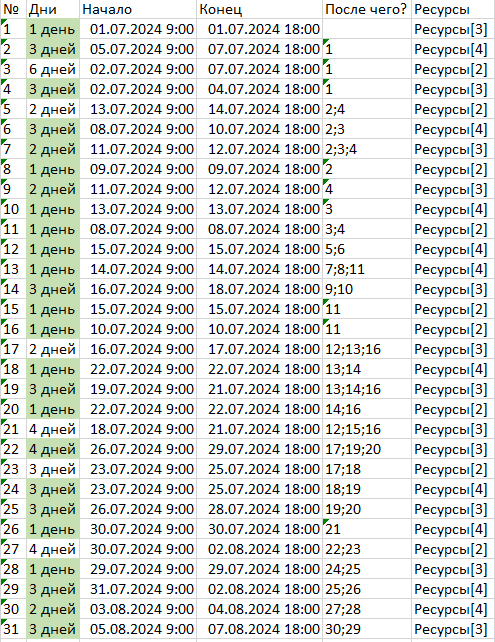
\includegraphics[height=0.6\textheight]{../img/1a2_days_change.png}\\ 
		Внешне кажется, что ничего не поменялось, но изменения есть.
		Их можно заметить, к примеру, посмотрев на задачи 6 и 11.\\
		{\LARGE Как это выглядит и сколько оно тратит:}\\
		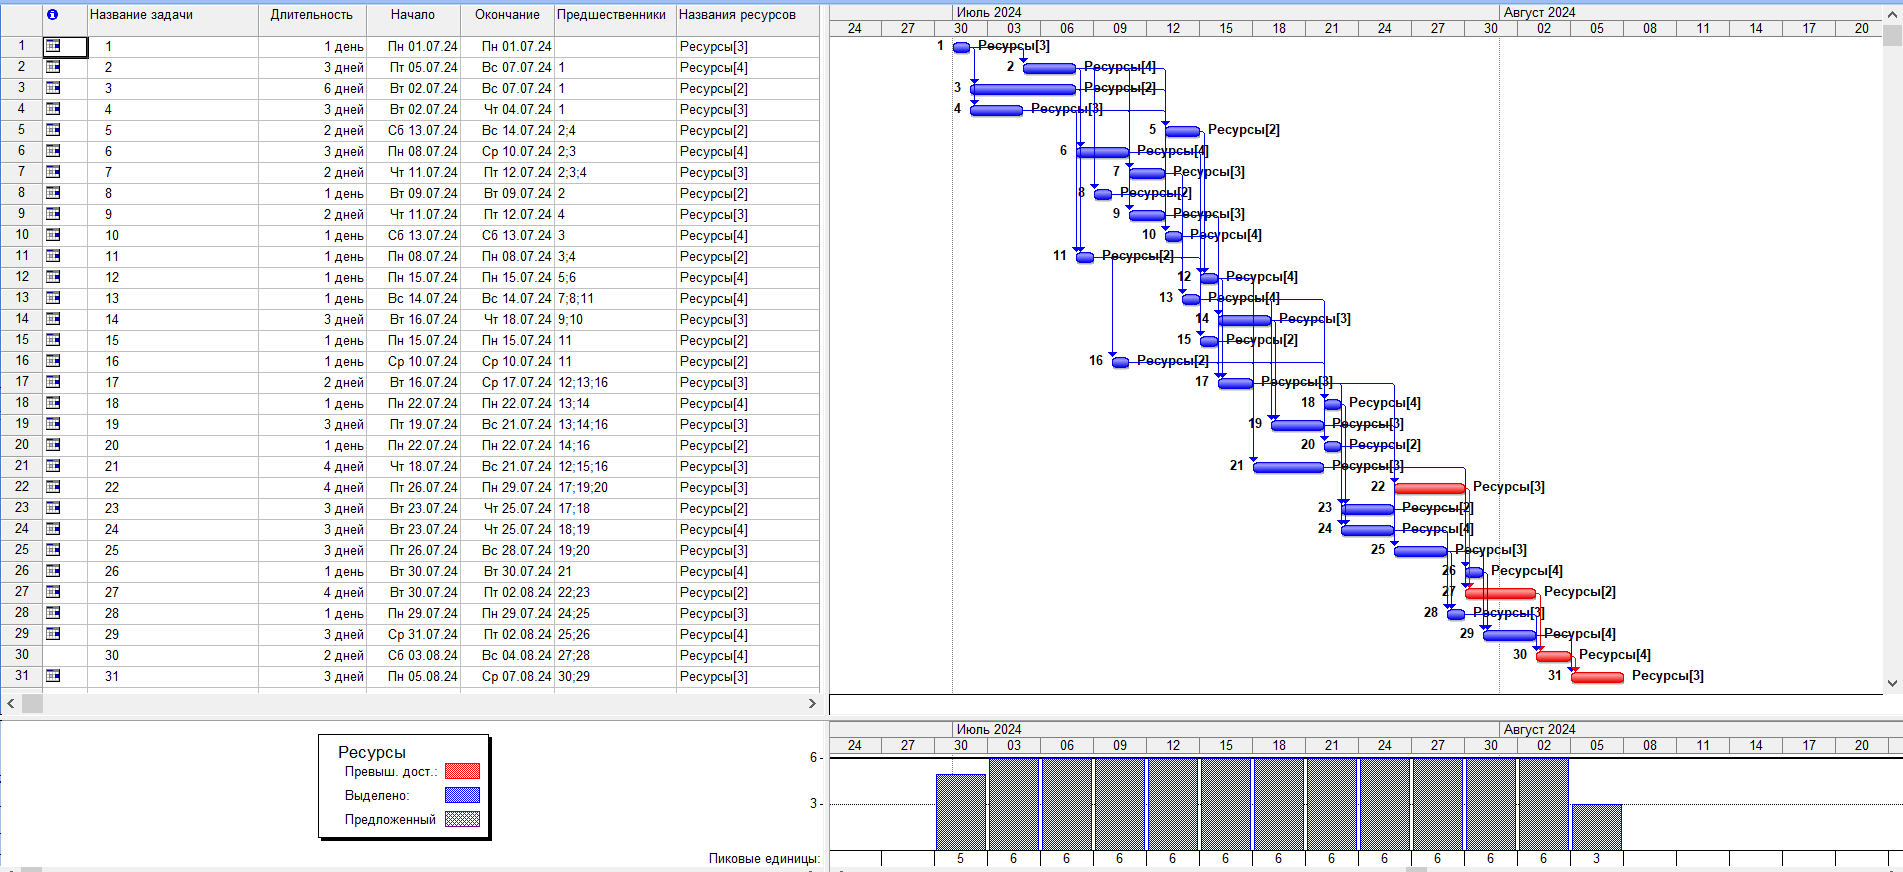
\includegraphics[width=\textwidth]{../img/1a2_answer.png}\\ 
	\subsection{Третий вариант}
		Покажем ещё какое-нибудь решение:
		{\LARGE Что поменяли:}\\
		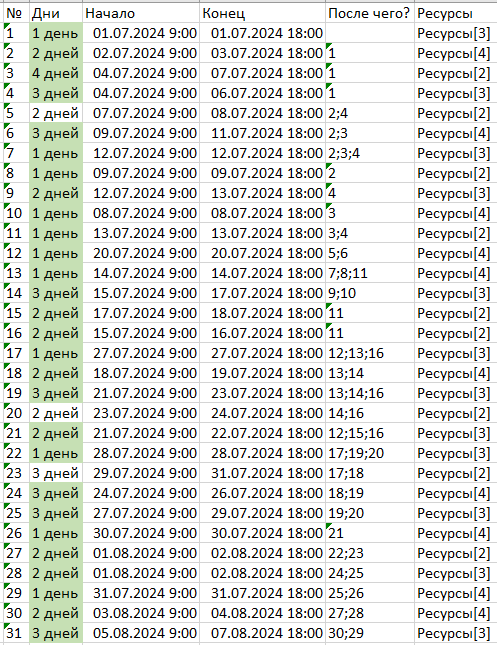
\includegraphics[height=0.6\textheight]{../img/1a3_days_change.png}\\ 
		{\LARGE Как это выглядит и сколько оно тратит:}\\
		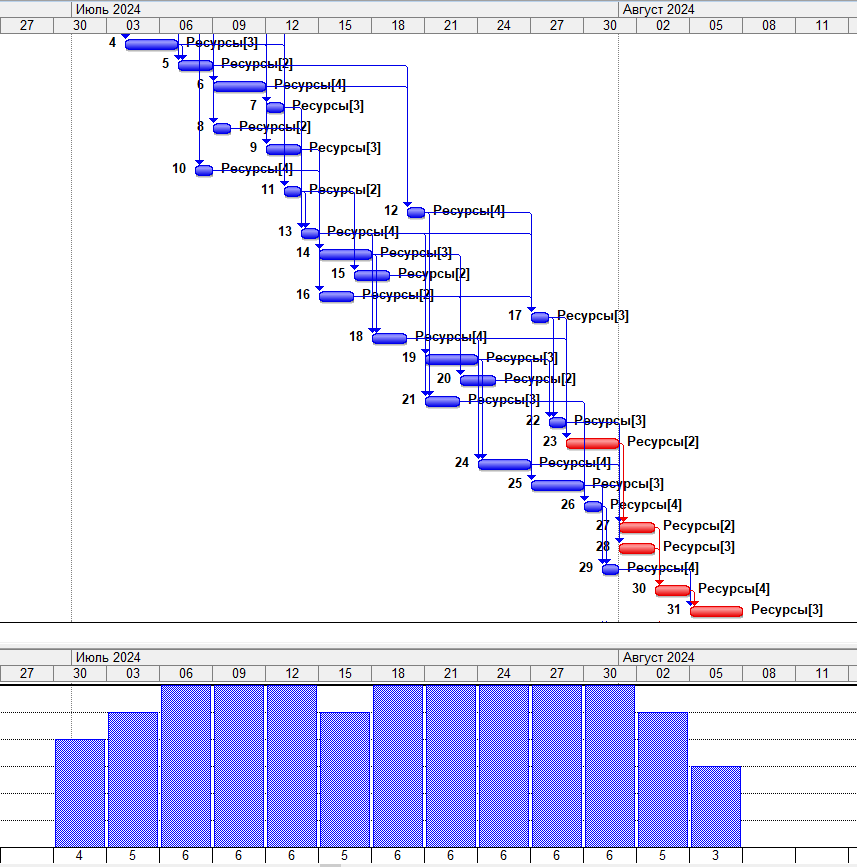
\includegraphics[width=\textwidth]{../img/1a3_answer.png}\\ 
\end{document}
